\documentclass[a4paper,10pt]{article}

\usepackage[hmargin={25mm,25mm},vmargin={25mm,25mm}]{geometry}
\usepackage{amsmath}
\usepackage{amsfonts}
\usepackage{graphicx}

\begin{document}

\begin{center}{\LARGE\bf
    The Auction Grinding Attack:} \\
  and a case for a liquidation penalty in dai
 
\end{center}

\section{Introduction}
This paper describes a potential economic attack vector on the automatic auction mechanisms in the multi-collateral dai system, in particular, the reversing collateral liquidation auction. In summary: an attacker could open a Collateralised Debt Position (CDP), take out a substantial amount of debt against their collateral, and intentionally allow the position to go unsafe, causing the collateral to go to the liquidation auction. Upon liquidation the attacker can bid on their own collateral's liquidation auction, following a deterministic (pure) bidding strategy, which I describe. Following this strategy leads to meaningful profits in the event that the auction's capital participation rate (CPR) turns out to be low. In the case with no CDP liquidation penalty, the attack is practically risk free, since the worst possible outcome for the attacker is their gas expense, which is essentially bounded and easily quantifiable in advance.
\par The key fact that permits this attack is that when a liquidation auction finishes ``in adequacy'', the excess collateral is returned to the owner of the CDP, meaning that when the CDP owner is bidding on their own auction in the surplus phase, the marginal cost of a new bid at any price is zero.
\par To make matters worse, provided the other bidders suspect that a liquidation might be an auction grinder's, the Nash equilibrium in the auction game (with the bidders as players) might be in favour of the attacker, since bidders may be deterred from participating, knowing that the grinder's strategy will preclude them from winning the auction.
\par In the presence of a non-zero liquidation penalty, the attacker will have a guaranteed up-front cost, meaning that the worst-case outcome is negative and the attack is no longer risk-free. I will provide a heuristic for setting the liquidation penalty that will deter a profit-seeking rational attacker; the heuristic will rely on a model of auction participation.

\section{The Collateral Auction}
The \emph{collateral auction} (also known as the {\tt flip}-auction), is one of the three auction types in the dai system. The other two are the \emph{debt auction} (the {\tt flop}-auction), and the \emph{surplus auction} (the {\tt flap}-auction). The collateral auction is used to sell off collateral from risky CDP positions in exchange for dai, to protect the system from excessive risk. When a CDP's status becomes unsafe, the system permits any agent to initiate a collateral auction, sending the collateral to the {\tt Flipper} contract, where it may receive bids. The mechanism used is a \emph{reversing auction}, which I now explain (details of the auction mechanism not relevant to the auction grinding attack are omitted).
\par Like the other two dai auction types, the collateral auction has two termination conditions. The first is that the auction will terminate after {\tt tau} seconds have passed from the moment the auction was initiated. The second is that {\tt ttl} seconds have passed from the moment of the last bid. When an auction has terminated, no more bids are accepted, and the winning bidder may claim their collateral from the contract. Both {\tt tau} and {\tt ttl} are risk parameters set by governance.
\par The goal of the collateral auction is to cover the outstanding dai debt on the liquidated CDP. Let {\tt tab} refer to the amount of dai debt outstanding on a CDP, and let {\tt ink} refer to the amount of collateral in the CDP, both at the moment of liquidation. Then, the first priority of the auction is to try to raise {\tt tab} dai, in exchange for any amount of the collateral, and if this much cannot be raised, to raise as much dai as possible.  The second priority of the auction is to treat the CDP owner fairly, by not liquidating more of their collateral than is necessary to cover the debt. These two priorities correspond to the two phases of the auction: called the {\tt tend} phase and the {\tt dent} phase.
\par In the {\tt tend} phase, the auction receives increasing bids (denoted {\tt bid}) of dai for the fixed amount {\tt ink} of collateral, with ${\tt bid} \leq {\tt tab}$. When a new, higher {\tt bid} is received, the difference between the new {\tt bid} and the previous {\tt bid} goes to the auction contract, while the rest goes to refund the previous bidder. If the auction terminates in the {\tt tend} phase (due to one of the two termination conditions above being met), all collateral goes to the winning bidder, and if in the end ${\tt bid} < {\tt tab}$ then we say the auction has \emph{finished in deficit}, and the deficit will need to be covered by an MKR-diluting debt auction.
\par The auction goes from the {\tt tend} phase to the {\tt dent} phase when it receives a {\tt bid} equal to {\tt tab}. In the {\tt dent} phase, the auction receives bids in the form of decreasing amounts of collateral (denoted {\tt lot}), with ${\tt lot} < {\tt ink}$. When a lower {\tt lot} is offered, {\tt tab} dai is transferred from the bidder to refund the previous bidder. When the auction terminates in the {\tt dent} phase, the bidder with the lowest {\tt lot} receives {\tt lot} collateral, and the CDP owner has ${\tt ink}-{\tt lot}$ collateral returned to them. When an auction finishes in the {\tt dent} phase, we say that the auction has \emph{finished in adequacy}, so no debt auction will be needed.

\par There are two key features of collateral auctions that create the possibility for the auction grinding attack: one concerning auctions that finish in deficit, and one concerning auctions that finish in surplus.
\par An auction that finishes in deficit will trigger an MKR dilution to cover the difference between the debt owed by the liquidated CDP and the dai raised in the collateral auction. Assuming the existence of a true value for the collateral, either the winner of the collateral auction has managed to buy collateral at a discount to the fair price, or at the time of liquidation the CDP's debt must have exceeded the value of its collateral (negative equity), or some combination of the two\footnote{There is also a possibility that the CDP has positive equity at the time of liquidation, as judged by the fair market value of the collateral, but due to a decline in the price of the collateral over the course of the auction, it could still finish in deficit. This additional ``basis risk'' that MKR capital is exposed to is not considered here.}. Hence, viewing this event as a ``value flow'', we see that the value of MKR capital flows to the auction winner (whose collateral purchase price is effectively subsidised), or the CDP debtor (whose excess debt over collateral value is forgiven), or both. The auction grinding attack will seek to exploit this value flow in the case that the CDP owner and the winning auction bidder are the same person.

\par An auction that finishes in surplus will have its excess collateral returned to the owner of the liquidated CDP. 
This means that (in the absence of a liquidation penalty) the marginal cost of a CDP owner placing a bid on the collateral auction of their own CDP is zero. The attack will exploit this fact in order to ensure that they can always win the auction.

\section{The Attack}
\par For the purposes of this section, we will assume there is no liquidation penalty. We will also neglect any risks associated with collateral price volatility during the course of the auction: the reason for this is that the attacker can choose to attempt this attack during a period when collateral price volatility is low. Moreover, they are free to hedge their exposure to the collateral externally to reduce their risk. It is also important that the attacker has extra dai available to them before they start the attack.
\par I now describe the attack: first the attacker must choose the collateral type that they wish to use for the attack. As we shall see, they may select the collateral type where they expect the least auction participation, or simply try the attack on all collateral types repeatedly. Let {\tt mat } be the liquidation ratio of the chosen collateral type, and we will call the collateral tokens of this collateral type gems. Let {\tt tab} and {\tt ink} be the amounts of dai debt and collateral gems, respectively, of the CDP upon liquidation.
\par Next, the attacker creates a CDP of this collateral type, deposits all of their gems, and borrows the maximum amount of dai from this CDP, hoping to get their position liquidated immediately. If their position does not become unsafe on the next collateral price feed update, they only have to draw more dai if possible, and wait until the next downward tick in the feed price. Once their CDP becomes unsafe, they initiate its liquidation, so the collateral auction will begin.
\par The attacker's strategy is simple: their first goal is to win their own collateral's liquidation auction, at the lowest price possible, with the auction finishing in deficit. Thus, they will place bids while the auction is in the {\tt tend} phase, hoping to win the auction\footnote{The exact strategy (choice of timing, bid increment, etc.) by which the bidder will attempt to win the auction in the {\tt tend} phase is up to the attacker.}. If the attacker is successful, winning the auction in the {\tt tend} phase paying {\tt bid} dai, we will have reached outcome $W({\tt bid})$. If someone thwarts this plan by outbidding them until the auction is in the {\tt dent} phase, then the attacker will abandon that plan and simply place another, final bid at the implied price corresponding to the attacker's view of the correct collateral value. At this point, one of two things will happen: either no one will outbid the attacker and they will win the auction, which we will call outcome $N$, or someone will outbid the attacker and end up buying (some of) the collateral at a premium to the attacker's notion of the fair value, which we will denote $Y({\tt lot})$ where {\tt lot} is the amount of gems bought by the winning bidder. In any case, the attacker guarantees that the auction will finish in one of the states $W({\tt bid})$, $N$, or $Y({\tt lot})$.
\par If the auction finishes in state $W({\tt bid})$, the attacker will have bought back their own collateral with less dai than they borrowed against it, ending with a profit.
\par If the auction finishes in state $N$, the attacker will have spent the same amount of dai that they just borrowed, and received in return the same amount of collateral that they put in (part of it going to them as the CDP owner, and part as the winner of the auction), so has made neither a profit nor a loss.
\par If the auction finishes in state $Y({\tt lot})$, the attacker will have effectively traded gems for dai with the winning bidder at a premium to their notion of the fair price, thus making a profit.
\begin{figure}
    \centering
%    \includegraphics[width=1.5in]{diag/atlasex1}
    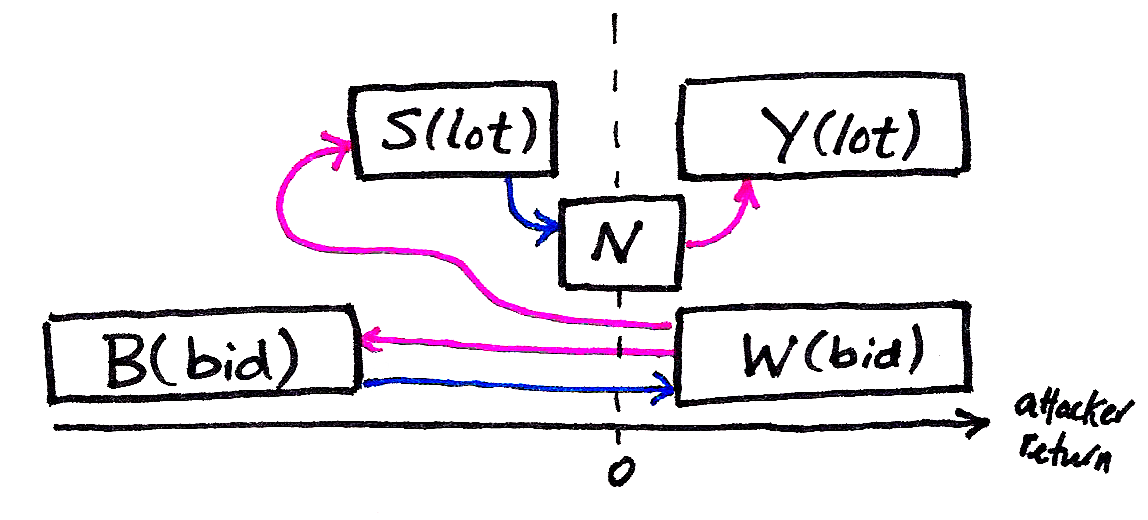
\includegraphics[width=3.5in]{gamegraph}
    \caption{Graph of attacker's strategy, where blue arrows depict moves that the attacker will make, and pink arrows depict moves that might be made by other auction participants. The horizontal position of a game state representing the total return for the attacker in the event that the auction terminates in that state.}
\end{figure}

We enumerate all relevant states of the auction, and display the game states as a graph in Figure 1:
\begin{description}
\item [$W({\tt bid})$] The auction is in the {\tt tend} phase and the attacker is the top bidder.
\item [$B({\tt bid})$] The auction is in the {\tt tend} phase and someone else is the top bidder.
\item [$N$] The auction is in the {\tt dent} phase and the attacker is the top bidder, having bid at most their fair price for the collateral.
\item [$S({\tt lot})$] The auction is in the {\tt dent} phase and someone else is the top bidder, having bid less than the attacker's fair price for the collateral.
\item [$Y({\tt lot})$] The auction is in the {\tt dent} phase and someone else is the top bidder, having bid more than the attacker's fair price for the collateral.
\end{description}
\par We also compute the attacker's return in case the auction finishes in each state, where return is calculated as the difference in the dai value between the attacker's starting and ending portfolio, assuming the attacker values one gem as {\tt wut} dai, and ignoring any gas costs, financing costs, and opportunity costs.
\begin{table}[h]
  \centering
\begin{tabular}{l{l}{l}r}
termination state & auction winner & attacker return \\
\hline
$W({\tt bid})$ & attacker & ${\tt tab} - {\tt bid}$ & $(>0)$  \\
$B({\tt bid})$ & other & ${\tt tab} - {\tt ink}\cdot{\tt wut}$ & $ (<0)$  \\
$N$            & attacker & $0$  \\
$S({\tt lot})$ & other & ${\tt tab} - {\tt lot}\cdot{\tt wut}$ & $(<0)$  \\
$Y({\tt lot})$ & other & ${\tt tab} - {\tt lot}\cdot{\tt wut}$ & $(>0)$  \\
\end{tabular}
\caption{Payoff table for auction grinding strategy with no liquidation penalty.}
\end{table}

\par As we have seen, the attacker can force the auction to finish in one of the three scenarios where their return is non-negative. Thus, provided one of the two scenarios where the return is positive could happen with non-negligible probability, the attacker will expect a positive expected return from following this strategy. In particular, the attacker can increase the chance of profiting through outcome $W({\tt bid})$ if they have sufficient capital to initiate a large liquidation (or many simultaneous liquidations) that many other market participants will be priced out of. Moreover, if the attacker ``griefs'' the system by following this strategy repeatedly and winning every auction, others may be discouraged from participating in future auctions (in game terms, the attacker is always able to force a draw, so competing bidders might choose not to play).

\newpage
\section{The Liquidation Penalty}
A natural approach to mitigating this attack is to add some friction to the liquidation process, in addition to the gas costs which are already present but may be too insignificant relative to the capital at play. I propose using the \emph{liquidation penalty} to this end. In short, a liquidation penalty is implemented by increasing the outstanding debt on a CDP by some factor {\tt axe} just as it goes to liquidation, so that a CDP that had {\tt tab} outstanding debt will be treated as if it had ${\tt axe} \cdot {\tt tab}$ of debt for the purposes of liquidation. {\tt axe} set to $1$ is equivalent to no liquidation penalty. The effect of this is that the CDP owner will get less of their collateral back at the end of a liquidation, since the auction would have been covering a greater debt: effectively, they have had an additional $({\tt axe} - 1) \cdot tab$ dai debited from their balance\footnote{There is an alternative way of implementing the liquidation penalty, by slashing a fraction of the collateral that is returned to the CDP owner at the end. It is straightforward to show that this method is completely equivalent to the one described above, for all parties involved.}.
\par We now recompute the payoff matrix on the auction grinding strategy when a liquidation penalty of {\tt axe} is used:
\begin{table}[h]
  \centering
\begin{tabular}{l{l}r}
termination state & attacker return \\
\hline
$W({\tt bid})$ &  ${\tt tab} - {\tt bid}$ & $(>0)$  \\
$B({\tt bid})$ & ${\tt tab} - {\tt ink}\cdot{\tt wut}$ & $ (<0)$  \\
$N$            &  $-({\tt axe} - 1) \cdot {\tt tab}$  & $(<0)$ \\
$S({\tt lot})$ &  ${\tt tab} - {\tt lot}\cdot{\tt wut}$ & $(<0)$  \\
$Y({\tt lot})$ &  ${\tt tab} - {\tt lot}\cdot{\tt wut}$ & $(>0)$  \\
\end{tabular}
\caption{Payoff table for auction grinding strategy with liquidation penalty set to {\tt axe}.}
\end{table}
\par The crucial difference is that now the attacker's strategy cannot guarantee that the attacker will not suffer losses from attempting the attack. Indeed, the previously neutral state $N$, where the attacker would have forced the game to go if they were unable to make a profit, now represents a loss for the attacker, and the attack is no longer risk-free. To discourage the attacker, it will be necessary to make their expected return negative by setting {\tt axe} sufficiently high, which requires some model of the probability of each auction outcome. We model this by taking a random variable $L \in [0, \infty ) $ for the implied price of the highest non-attacker bid, assuming this to be independent of the attacker's presence and behaviour: the distribution of this random variable should capture the attacker's expectation that they will be challenged by another bidder in the auction. Integrating over probabilities $\mathbb{P}(L = l)$ and splitting the integral over the three possible termination states of the auctions gives the attacker's expected return:
\begin{equation*}
  \mathbb{E} = \int_{l = 0}^{\frac{\tt tab}{\tt ink}} ({\tt tab} - l \cdot {\tt ink})\cdot \mathbb{P}(L = l) \mathrm{d}l - \int_{l = \frac{\tt tab}{\tt ink}}^{\tt wut} ({\tt axe} - 1)\cdot {\tt tab} \cdot \mathbb{P}(L = l) \mathrm{d}l + \int_{l = {\tt wut}}^{\infty} (1 - \frac{{\tt axe} \cdot {\tt wut}}{l})\cdot {\tt tab} \cdot \mathbb{P}(L = l) \mathrm{d}l
\end{equation*}
whenever ${\tt axe} < \frac{{\tt wut} \cdot {\tt lot}}{\tt tab}$, and
\begin{equation*}
\mathbb{E} = \int_{l = 0}^{\tt wut} ({\tt tab} - l \cdot {\tt ink})\cdot \mathbb{P}(L = l) \mathrm{d}l + \int_{l = {\tt wut}}^{\frac{{\tt axe}\cdot{\tt tab}}{\tt lot}} ({\tt tab} - {\tt ink}\cdot {\tt wut}) \cdot \mathbb{P}(L = l) \mathrm{d}l + \int_{l = \frac{{\tt axe}\cdot{\tt tab}}{\tt lot}}^{\infty} (1 - \frac{{\tt axe}\cdot{\tt wut}}{l})\cdot {\tt tab} \cdot \mathbb{P}(L = l) \mathrm{d}l
\end{equation*}
when ${\tt axe} >= \frac{{\tt wut} \cdot {\tt lot}}{\tt tab}$.
\par Thus, assuming a model of non-attacker auction participation in the form of a probability distribution for $L$, we can determine the minimum {\tt axe} for which the attacker's expected return is negative. Initially, we can use a heuristic to estimate this probability distribution, and after the auctions have been running for some time we can use empirical data to adjust our model, repeat the computation, and determine if {\tt axe} should be increased or decreased.
\par As an example, we can take a generalised student's t-distribution for $L$, with mean ${\tt r \cdot wut}$ (where $r$ is some auction discount constant), scaling parameter $\frac{1}{20}{\tt wut}$, and one degree of freedom. An example of the probability density function, along with the attacker's profit, are shown in Figure 2. By numerically integrating the above expressions for the attacker's expected return with this distribution, taking ${\tt wut} = 500$, $r = 0.95$, ${\tt tab} = 10000$, ${\tt ink} = 30$, we find that in order to make the expected return negative we must set ${\tt axe} > 1.0835$ (i.e. we must apply a liquidation penalty of at least 8.35\% the value of the outstanding debt).

\begin{figure}[h]
    \centering
%    \includegraphics[width=1.5in]{diag/atlasex1}
    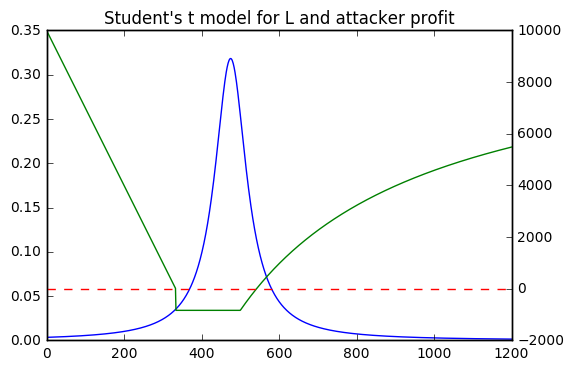
\includegraphics[width=4.5in]{tgraph}
    \caption{The probability density function of the t-distribution model for $L$, with ${\tt wut} = 500$ and $r = 0.95$ (corresponding to a mean auction price discount of 5\%). Also plotted is the attacker's profit as a function of $L$, where we have set ${\tt tab} = 10000$, ${\tt ink} = 30$, and ${\tt axe} = 1.0835$}
\end{figure}

The above heuristic assumes that $L$ is independent of the attacker's behaviour, and in particular that the attacker is not able to predict $L$ ahead of time. This assumption is flawed, since a motivated attacker is likely to strike during a regime where liquidity is stretched, by observing market conditions before initiating the liquidation. Moreover, the attacker can influence liquidity conditions themselves, either by manipulating the market in some way, or simply by attempting this attack with a very large amount of debt. Therefore, the heuristic above should be used very conservatively, choosing a more pessimistic (worst-case) model for $L$ if possible.

\section{Conclusion}
\par In the discussion above, I have explained the necessity of the liquidation penalty, without which the collateral auctions are vulnerable to an unpleasant economic attack. With an appropriately chosen liquidation penalty, determined by estimating the expected collateral auction participation (or based on existing data), the attacker will no longer expect a profit from the attack, and will be deterred from attempting it in normal conditions. There remains a risk that this attack could be profitably executed by a well-capitalised attacker who times their liquidation to occur during a moment of extreme market stress, where for some reason auction participation is much lower than expected. This possibility should be kept in mind as a potential black swan risk, and will be the subject of future research.
\end{document}
